\documentclass[usenames,dvipsnames]{beamer}
\usepackage[utf8]{inputenc}
\usepackage[T1]{fontenc}
\usepackage[francais]{babel}
\usepackage{xcolor}
\usepackage{packages/tikz-uml}
% \usepackage[amsthm]{ntheorem} %theorems and co.
\usetheme{Singapore} %Boadilla | Bergen | Madrid | Antibes | Hannover | Singapore | Warsaw
 
%----------------------------------------------------------------------------------------
%   TITLE INFORMATION
%----------------------------------------------------------------------------------------
\title{LaRuche}
\subtitle{HLSE602 -- Projet CMI Annuel}
\author{B. Rima \and O. Farajallah \and W. Soussi}
\institute[UM]{L3 CMI Informatique}
\date{\today}

\begin{document}
%----------------------------------------------------------------------------------------
%   TITLE FRAME
%----------------------------------------------------------------------------------------
\begin{frame}
\titlepage
\end{frame}
%----------------------------------------------------------------------------------------
%   OUTLINE
%----------------------------------------------------------------------------------------
\begin{frame}{Sommaire}
\tableofcontents
\end{frame}
%----------------------------------------------------------------------------------------
%   INTRODUCTION
%----------------------------------------------------------------------------------------
\section{Introduction}
\begin{frame}{Contexte du projet}{Introduction}
  \begin{description}
    \item [Projet CMI :] Module d'un projet annuel pour l'année 2017--2018 dans le cadre du \textbf{CMI Informatique}.
    \item [Responsable CMI Informatique :] Mme Anne-Elisabeth Baert.
    \item [Tuteur et Encadrant du projet :] M. Eric Bourreau.
    \item [Lieux de travail :] La \textbf{FDS} et le \textbf{LIRMM}.
  \end{description}
\end{frame}

%----------------------------------------------------------------------------------------
%   PROBLÉMATIQUE ET MÉTHODOLOGIE DE RÉSOLUTION
%----------------------------------------------------------------------------------------
\section{Problématique et Méthodologie de Résolution}
\subsection{Problématique}
\begin{frame}{Problématique}{Problématique et Méthodologie de Résolution}
\begin{columns}[onlytextwidth, T]
  \column{55mm}
    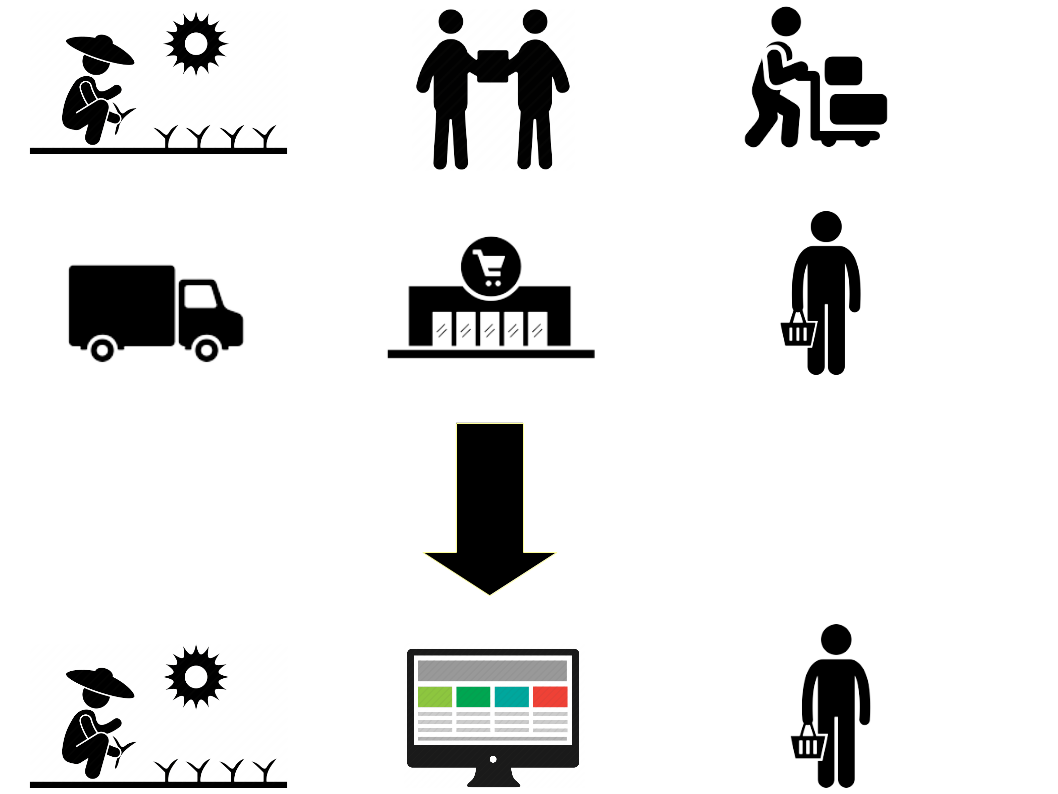
\includegraphics[scale=0.2]{images/chain_production.png}

  \column{\dimexpr\linewidth-40mm-2mm}
    \begin{block}{Consommateurs :}
    Acheter des produits frais et minimiser les étapes de processing.
    \end{block}

    \begin{block}{Producteurs :}
    Se libérer des centres d'achat et des intermédiaires de distribution.
    \end{block}
\end{columns}
  % \begin{figure}[!ht]
  %   \centering
  %   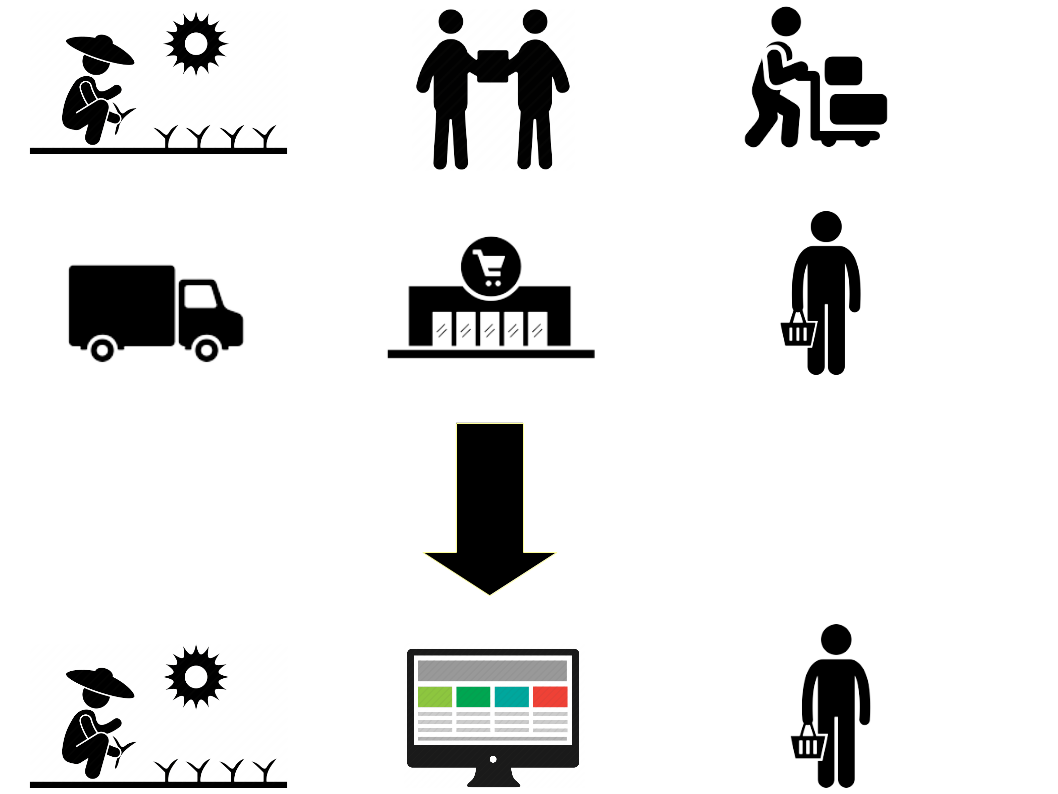
\includegraphics[scale=0.2]{images/chain_production.png}
  % \end{figure}
  % \begin{description}
  %   \item[Consommateurs :] acheter des produits frais et minimiser les étapes de processing.
  %   \item[Producteurs :] se libérer des centres d'achat et des intermédiaires de distribution.
  % \end{description}
\end{frame}

\subsection{Solutions}
\begin{frame}{Solution possible : La Ruche Qui Dit Oui}{Problématique et Méthodologie de Résolution}
\begin{block}{Site Web}
Une interface directe entre \textbf{consommateurs} et \textbf{fournisseurs}.
\end{block}

\begin{definition}[Ruche]
Un regroupement de plusieurs membres \textbf{consommateurs} et \textbf{fournisseurs} d'une région, guidé par un \textbf{responsable de ruche}.
\end{definition}

\begin{block}{Vision Centralisée}
\begin{itemize}
  \item l'ensemble des ruches obeit à une \textbf{Ruche-Mama}.
  \item les besoins de chaque ruche sont transmis à la \textbf{Ruche-Mama} via le responsable de ruche correspondant.
  \item la \textbf{Ruche-Mama} s'occupe de la gestion des ruches : création, réglementations internes, interactions, évolution et extensibilité des services, $\dots$.
\end{itemize}
\end{block}
\end{frame}

\begin{frame}{Solution proposée : \texttt{LaRuche}}{Problématique et Méthodologie de Résolution}
\begin{block}{Site Web}
Une interface directe entre \textbf{consommateurs} et \textbf{fournisseurs}.
\end{block}

\begin{definition}[Ruche]
Un regroupement de plusieurs \textbf{fournisseurs} d'une région, \textbf{sans guide explicite} préfixé par le site.
\end{definition}

\begin{block}{Vision Décentralisée et Autonome}
\begin{itemize}
  \item l'ensemble des ruches ne répond à \textbf{aucune entité centralisée fédéral}.
  \item chaque ruche s'occupe de ses propres besoins et de leur gestion sans besoin d'un intermédiaire et d'une hiérarchie autoritaire à respecter.
\end{itemize}
\end{block}
\end{frame}

\subsection{Méthodes agiles}
\begin{frame}{Méthodologie de résolution : méthodes agiles}{Problématique et Méthodologie de Résolution}
\begin{block}{Méthodes Agiles}
Une approche de développement logiciel de plus en plus prépondérante basée sur une conception/développement itérative, orientée-test et orientée-client.
\end{block}

\begin{block}{Pourquoi ?}
\begin{itemize}
  \item meilleure gestion des ressources
  \item sortie plus fréquente de versions fonctionnelles et testées du produit
  \item interaction plus fréquente avec les clients : adaptation et extensibilité du produit selon leurs besoins
\end{itemize}
\end{block}
\end{frame}
%----------------------------------------------------------------------------------------
%   CONCEPTION
%----------------------------------------------------------------------------------------
\section{Conception}
\subsection{Outils de conception utilisés}
\begin{frame}{Outils de conception utilisés}{Conception}
\begin{block}{Diagrammes de cas d'usage}
Des diagrammes dynamiques, souvent utilisés en \textbf{UML} pour décrire en haut niveau des fonctionnalités d'un système.
\end{block}

\begin{block}{Modèle EA}
Un modèle \textbf{conceptuel} utilisé pour décrire les entités du projet et les associations décrivant leurs relations et comportements.
\end{block}

\begin{block}{Schéma de base de données}
Un schéma en modèle \textbf{relationnel} traduit à partir du \textbf{modèle EA} et servant comme \textbf{support} lors de l'implémentation de la \textbf{base de données}.
\end{block}

\begin{block}{\textit{mockup storyboard}}
Un document de haut niveau (peu de détails sur les fonctionnalités) pour schématiser l'utilisation d'un projet.
\end{block}
\end{frame}

\subsection{\protect\textit{User Stories} : outil de conception agile}
\begin{frame}{\textit{User Stories} : outil de conception agile}{Conception}
\begin{block}{\textit{User Stories}}
Des requis fournis par les clients, décrivant en langage naturel les fonctionnalités qu'ils souhaitent avoir dans le produit développé.
\end{block}

\begin{block}{\textcolor{Sepia}{\texttt{Intitulé}}}
\begin{it}
  En tant que \textcolor{DarkOrchid}{\texttt{<rôle>}}, je souhaite \textcolor{BrickRed}{\texttt{<fonctionnalité>}}, \\
  ~~~~~~~~~dans le but de \textcolor{OliveGreen}{\texttt{<bénéfice>}}.
\end{it}
\end{block}
\end{frame}

\subsection{Côté fournisseur}
\begin{frame}{Côté fournisseur}{Conception}
\begin{block}{Besoins}
\begin{enumerate}
  \item Un profil d'utilisateur \textbf{fournisseur} : propriétés et fonctionnalités via des \textit{user-stories}.
  \item Une \textbf{structure de données} pour décrire le \textbf{regroupement des fournisseurs} et leurs \textbf{interactions} : \texttt{ruche}, \texttt{opérateur cellule}, \texttt{voisins}, $\dots$
\end{enumerate}
\end{block}
\end{frame}

\subsubsection*{\protect\textit{User-stories} des fournisseurs}
\begin{frame}{Intitulés des \textit{user-stories} fournisseurs}{Côté fournisseur}
\begin{enumerate}
  \item Définition et stockage de produits.
  \item Offre de Paniers.
  \item Rapports de suivi périodiques.
  \item Politique de rupture des stocks.
  \item Politique de partage intracellulaire dans une ruche.
  \item Validation de commandes.
  \item Attribution de factures.
\end{enumerate}
\end{frame}

\begin{frame}{Exemple d'une \textit{user-story} fournisseur}{Côté fournisseur}
\begin{block}{\textcolor{Sepia}{\texttt{Définition et stockage de produits}}}
En tant que \textcolor{DarkOrchid}{fournisseur}, je souhaite {\color{BrickRed} \textbf{définir} ma \textbf{sélection de produits} selon des \textbf{informations caractéristiques} à fournir dans des \textbf{formulaires}},\\
~~~~~~~~~dans le but de {\color{OliveGreen}maximiser la transparence de mes produits pour gagner la fidelité de mes clients, tout en \textbf{gérant} (création, modification, ajout, suppression) ma sélection à travers le site}.
\end{block}
\end{frame}

\subsubsection*{Profil fournisseur}
\begin{frame}{Profil fournisseur}{Côté fournisseur}
\begin{enumerate}
  \item Un fournisseur offre des produits/paniers de produits divers.
  \item Un fournisseur gére ses produits/paniers dans des stocks.
  \item Un fournisseur suit l'évolution de ses ressources via des rapports de suivi périodiques.
  \item Un fournisseur interagit avec d'autres fournisseurs pour créer des ruches et organiser des évènements de collecte et uniquement avec des clients qui l'ont déjà contacté.
  \item Un fournisseur valide les commandes de réservation des produits.
  \item Un fournisseur règle les commandes physiquement, en premier temps, et puis via le site dans les versions ultérieures.
  \item Un fournisseur imprime les factures, créées par le site lors de la réservation des produits par des clients, et les émet aux clients correspondants lors de la collecte de leurs produits.
\end{enumerate}
\end{frame}

\begin{frame}{Exemple d'un diagramme de cas d'usage (version de base)}{Côté fournisseur}
\begin{figure}[!ht]
  \centering
  \resizebox{0.75\textwidth}{!}{
    \begin{tikzpicture}
      \setcounter{tikzumlUseCaseNum}{0}
      \umlactor[x=-1, y=-1]{Vendor}
      \umlactor[x=8, y=-1]{Database}
      \begin{umlsystem}[x=3, fill=green!10]{home page}
        \umlusecase[width=3cm]{Add/Delete/Modify Products}
        \umlusecase[y=-2.5, width=3cm]{Add/Delete/Modify Baskets}
        \umlusecase[y=-4.5]{Check Stocks}
        \umlusecase[y=-6.5]{Check Reports}
      \end{umlsystem}
      \umlextend[name=ext]{usecase-2}{usecase-1}
      \umlextend{usecase-4}{usecase-3}
      \umlassoc{Vendor}{usecase-1}
      \umlassoc{Vendor}{usecase-2}
      \umlassoc{Vendor}{usecase-3}
      \umlassoc{Vendor}{usecase-4}
      \umlassoc{Database}{usecase-1}
      \umlassoc{Database}{usecase-2}
      \umlassoc{Database}{usecase-3}
      \umlassoc{Database}{usecase-4}
      \umlnote[x=-2, y=-4]{ext-1}{Products have to exist in the database prior to the introduction of baskets}
    \end{tikzpicture}
  }
\end{figure}
\end{frame}

\begin{frame}{Exemple d'un diagramme de cas d'usage (version ultérieure)}{Côté fournisseur}
\begin{figure}[!ht]
  \centering
  \resizebox{0.65\textwidth}{!}{
    \begin{tikzpicture}
      \setcounter{tikzumlUseCaseNum}{0}
      \umlactor{Vendor}
      \umlactor[x=12, y=-2]{Database}
      \umlactor[y=-13]{Client User Database}
      \umlactor[x=12, y=-11]{Bill Reception Platform}
      \umlactor[x=4.5, y=-13]{Bank/PayPal}
      \begin{umlsystem}[x=4, fill=red!10]{vendor home page}
        \umlusecase[width=2cm]{Check Stocks}
        \umlusecase[x=5, width=2cm]{Allow Delayed Orders}
        \umlusecase[x=2.6, y=-3, width=3cm]{Set Purchase Deadline}
        \umlusecase[x=4, y=-6, width=3cm]{Check Pending Orders}
        \umlusecase[y=-8, width=2cm]{Process Pending Orders}
        \umlusecase[x=5, y=-8, width=2cm]{Send Bill}
        \umlusecase[x=4.5, y=-11, width=2cm]{Update Sales' History}
      \end{umlsystem}
      \umlextend{usecase-2}{usecase-1}
      \umlextend[name=deadline]{usecase-3}{usecase-4}
      \umlextend[name=checkPending1]{usecase-4}{usecase-5}
      \umlinclude{usecase-5}{usecase-6}
      \umlinclude{usecase-6}{usecase-7}
      \umlassoc{Vendor}{usecase-1}
      \umlassoc[name=checkPending2]{Vendor}{usecase-4}
      \umlassoc[name=process]{Vendor}{usecase-5}
      \umlassoc{Database}{usecase-2}
      \umlassoc{Database}{usecase-3}
      \umlassoc{Database}{usecase-4}
      \umlassoc{Database}{usecase-7}
      \umlassoc{Bill Reception Platform}{usecase-6}
      \umlassoc{Bank/PayPal}{usecase-6}
      \umlassoc{Client User Database}{usecase-6}
      \umlnote[x=-0.5, y=-5]{checkPending1-1}{only if validating transactions is set to manual}
      \umlnote[x=-0.5, y=-5]{checkPending2-1}{only if validating transactions is set to manual}
      \umlnote[x=-0.5, y=-8]{process-1}{only if validating transactions is set to automatic}
      \umlnote[x=-0.5, y=-11]{deadline-1}{according to the number of pending orders}
    \end{tikzpicture}
  }
\end{figure}
\end{frame}

\subsubsection*{Ruche : Structure de données proposée}
\begin{frame}{Ruche : Structure de données proposée}{Côté fournisseur}
\begin{block}{Définitions de base}
\begin{description}
  \item[$\textbf{V}$]{ensemble des fournisseurs.}
  \item[$\textbf{C}$]{ensemble des clients.}
  \item[$\pi_v$]{\textbf{opérateur} appliqué à $v \in V$ désignant une \textbf{cellule}, c.à.d. un \textbf{cercle} dont le centre est le point représentant les coordonnées du fournisseur $v$ et dont le rayon est la distance maximale en \textbf{km} qu'il souhaite parcourir afin de se rendre à un lieu de collecte.}
\end{description}
\end{block}
\end{frame}

\begin{frame}{Ruche : Structure de données proposée($2$)}{Côté fournisseur}
\begin{block}{Ruche}
Soit $v_1, v_2, \dots, v_n \in V^n$. Une \textbf{ruche} $R = (p, V_R)$ est composée de :
\begin{description}
  \item[$\mathbf{V_R}$]{ensemble de fournisseurs dont les cellules s'intersectent;}
  \item[$\mathbf{p}$]{un point de collecte obtenu à partir d'une opération\footnote{le choix du point est relatif aux fournisseurs de la ruche, étant indéterministe en soi} sur la zone d'intersection des cellules correspondantes aux vendeurs de $V$.}
\end{description}
Autrement dit, $R = \{p, \{v_1, v_2, \dots, v_n \in V\; |\; \pi_{v_1} \cap \pi_{v_2} \cap \dots \cap \pi_{v_2} \neq \varnothing\}\}$
\end{block}
\end{frame}

\begin{frame}{Ruche : Structure de données proposée($3$)}{Côté fournisseur}
\begin{figure}[!ht]
  \centering
  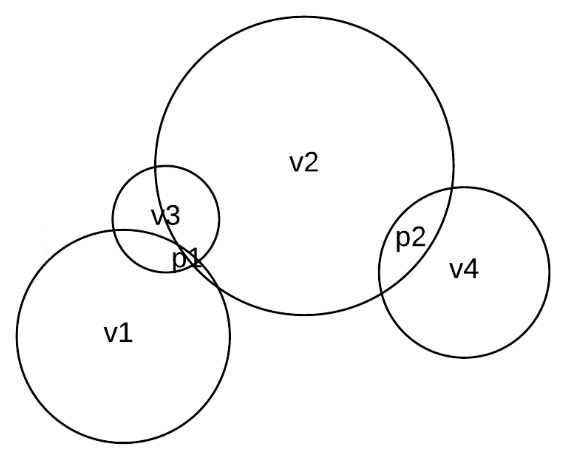
\includegraphics[scale=0.17]{images/exemple_introductif1.png}
\end{figure}

\begin{block}{Appartenance Simultanée}
Un fournisseur peut appartenir à plusieurs ruches simultanément.
\end{block}

\begin{block}{Fournisseurs Voisins}
Soit $R = \{p, V_R\}$ une ruche. Deux fournisseurs $v_1$ et $v_2$ sont dits \textbf{voisins} $\iff v_1 \in V_R\; \text{et}\; v_2 \in V_R$. On note $\texttt{Voisins}(v)$ l'\textbf{ensemble des voisins} d'un fournisseur $v$, contenant \textbf{tous les voisins} de \textbf{toutes les ruches} auxquelles il appartient.
\end{block}
\end{frame}

\begin{frame}{Ruche : Structure de données proposée($4$)}{Côté fournisseur}
\begin{figure}[!ht]
  \centering
  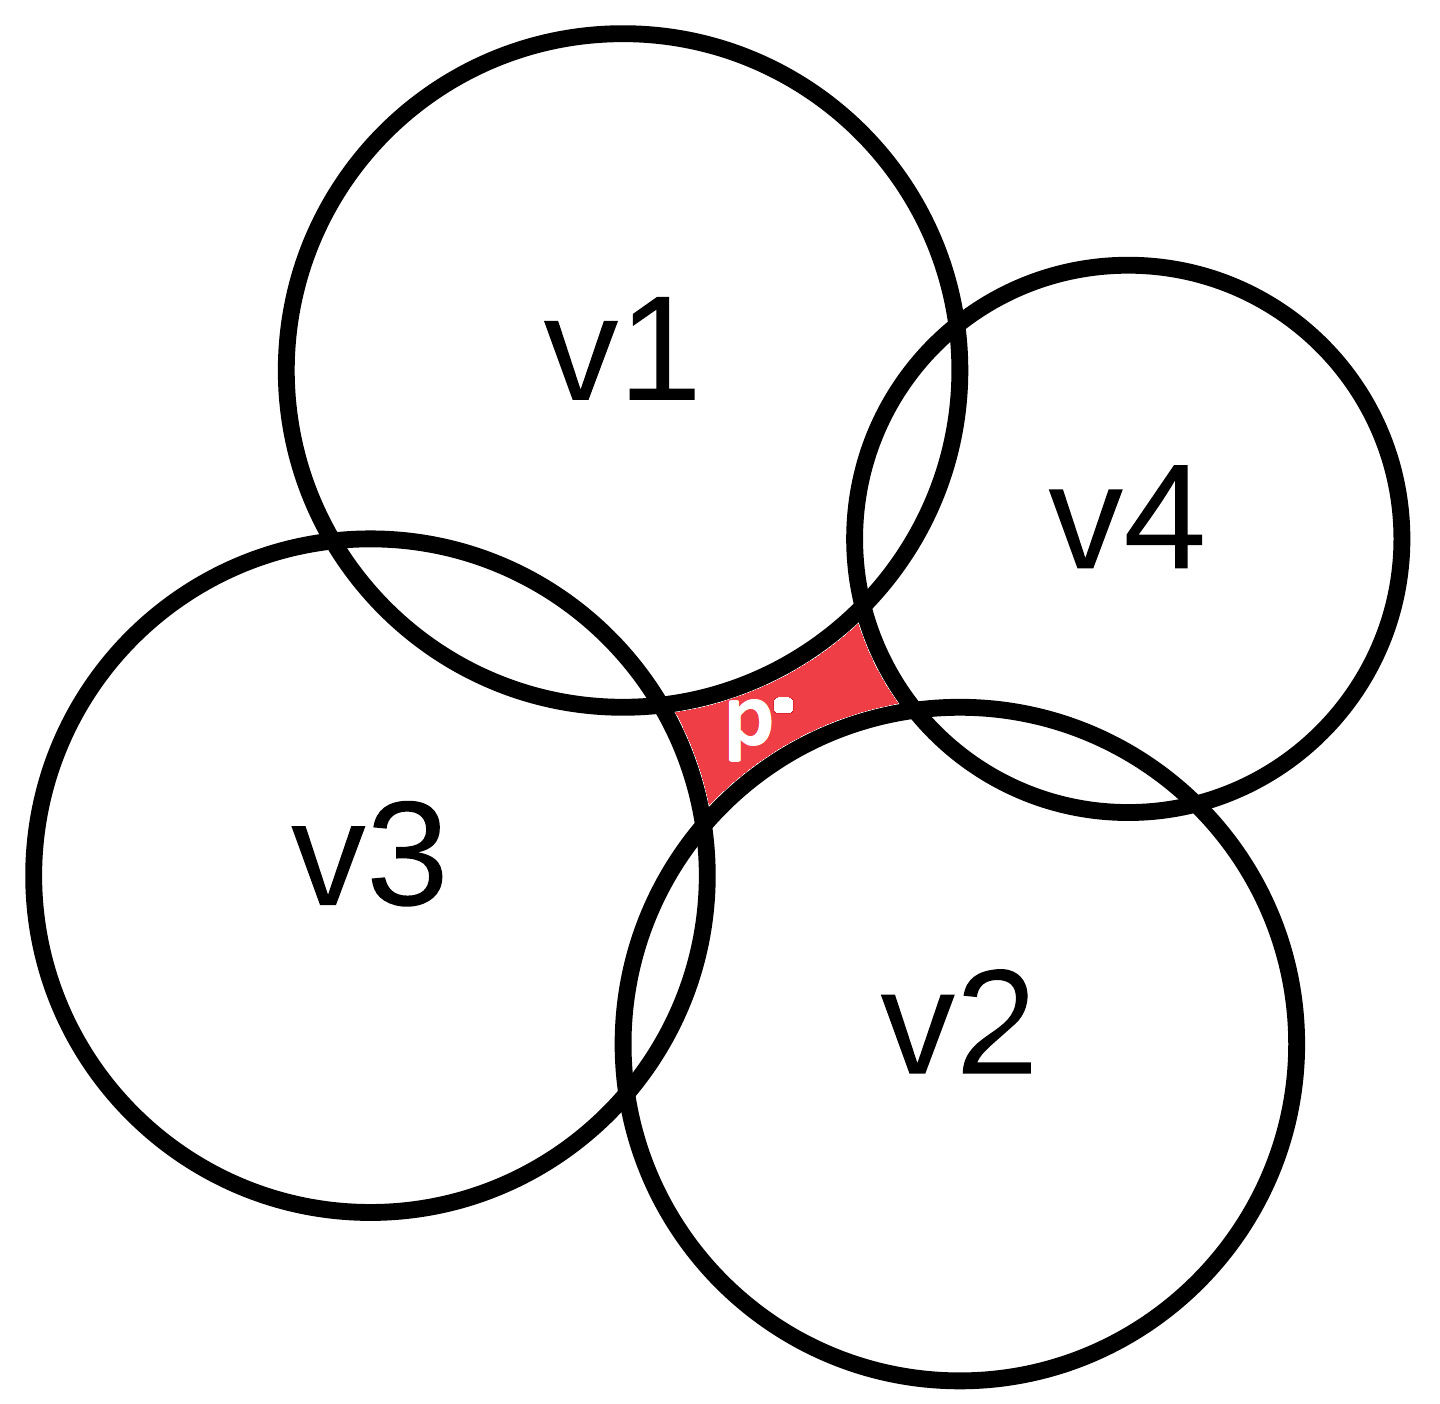
\includegraphics[scale=0.08]{images/exemple_introductif2.png}
\end{figure}

\begin{block}{Voisinage Imposé}
Soient $v_1$ et $v_2$ deux fournisseurs tels que $v_2 \notin \texttt{Voisins}(v_1)$. S'il existe des fournisseurs $v_3$ et $v_4$ tels que $v_3, v_4 \in \texttt{Voisins}(v_1) \cap \texttt{Voisins}(v_2)$ et $v_3 \notin \texttt{Voisins}(v_4)$, alors il existe une ruche plus optimale contenant $v_1, v_2, v_3\; \text{et}\; v_4$ que les ruches séparées les contenant.
\end{block}
\end{frame}

\subsection{Côté client}


% TODO:
%  need to fix the umlassoc
% 
% 
\begin{frame}{Côté client}{Conception}
  \begin{figure}[!ht]
    \resizebox{0.65\textwidth}{!}{
      \begin{tikzpicture}
        \umlactor{User}
        \umlactor[x=12, y=-1]{Database}
        \begin{umlsystem}[x=4, fill=red!10]{index page}
          \umlusecase{Sign-up}
          \umlusecase[y=-2]{Sign-in}
          \umlusecase[x=4, width=1.5cm]{Create database entry}
          \umlusecase[x=4, y=-3, width=1.5cm]{Verify credentials}
          \umlusecase[y=-4]{Footer menu}
        \end{umlsystem}
        \umlassoc{User}{usecase-1}
        \umlassoc{User}{usecase-2}
        % \umlassoc{User}{usecase-5}
        \umlassoc{Database}{usecase-3}
        \umlassoc{Database}{usecase-4}
        \umlinclude{usecase-1}{usecase-3}
        \umlinclude{usecase-2}{usecase-4}
        \umlinclude{usecase-3}{usecase-4}
      \end{tikzpicture}
    }
  \end{figure}
\end{frame}




\begin{frame}{Côté client}{Conception}
  \begin{figure}[!ht]
    \centering
    \resizebox{0.65\textwidth}{!}{
    \begin{tikzpicture}
      \setcounter{tikzumlUseCaseNum}{0}
      \umlactor{User}
      \umlactor[y=-4]{Vendor}
      \umlactor[x=10, y=-3]{Database}
      \begin{umlsystem}[x=4, fill=green!10]{home page}
        \umlusecase[x=1, width=3cm]{Display Products/Collection Events}
        \umlusecase[x=1, y=-3, width=3cm]{Display Stock/Hive Information}
        \umlusecase[x=1, y=-5]{Search}
        \umlusecase[x=1, y=-7]{Footer menu}
      \end{umlsystem}
      \umlinherit{Vendor}{User}
      \umlextend{usecase-2}{usecase-1}
      \umlassoc{User}{usecase-1}
      \umlassoc{Vendor}{usecase-2}
      \umlassoc{User}{usecase-3}
      \umlassoc{User}{usecase-4}
      \umlassoc{Database}{usecase-1}
      \umlassoc{Database}{usecase-3}
    \end{tikzpicture}
    }
  \end{figure}
  
\end{frame}



\begin{frame}{Côté client}{Conception}
  \begin{figure}[!ht]
   \centering
   \resizebox{0.65\textwidth}{!}{
     \begin{tikzpicture}
       \setcounter{tikzumlUseCaseNum}{0}
       \umlactor{Vendor}
       \umlactor[x=12, y=-2]{Database}
       \umlactor[y=-13]{Client User Database}
       \umlactor[x=12, y=-11]{Bill Reception Platform}
       \umlactor[x=4.5, y=-13]{Bank/PayPal}
       \begin{umlsystem}[x=4, fill=red!10]{vendor home page}
         \umlusecase[width=2cm]{Check Stocks}
         \umlusecase[x=5, width=2cm]{Allow Delayed Orders}
         \umlusecase[x=2.6, y=-3, width=3cm]{Set Purchase Deadline}
         \umlusecase[x=4, y=-6, width=3cm]{Check Pending Orders}
         \umlusecase[y=-8, width=2cm]{Process Pending Orders}
         \umlusecase[x=5, y=-8, width=2cm]{Send Bill}
         \umlusecase[x=4.5, y=-11, width=2cm]{Update Sales' History}
       \end{umlsystem}
       \umlextend{usecase-2}{usecase-1}
       \umlextend[name=deadline]{usecase-3}{usecase-4}
       \umlextend[name=checkPending1]{usecase-4}{usecase-5}
       \umlinclude{usecase-5}{usecase-6}
       \umlinclude{usecase-6}{usecase-7}
       \umlassoc{Vendor}{usecase-1}
       \umlassoc[name=checkPending2]{Vendor}{usecase-4}
       \umlassoc[name=process]{Vendor}{usecase-5}
       \umlassoc{Database}{usecase-2}
       \umlassoc{Database}{usecase-3}
       \umlassoc{Database}{usecase-4}
       \umlassoc{Database}{usecase-7}
       \umlassoc{Bill Reception Platform}{usecase-6}
       \umlassoc{Bank/PayPal}{usecase-6}
       \umlassoc{Client User Database}{usecase-6}
       \umlnote[x=-0.5, y=-5]{checkPending1-1}{only if validating transactions is set to manual}
       \umlnote[x=-0.5, y=-5]{checkPending2-1}{only if validating transactions is set to manual}
       \umlnote[x=-0.5, y=-8]{process-1}{only if validating transactions is set to automatic}
       \umlnote[x=-0.5, y=-11]{deadline-1}{according to the number of pending orders}
     \end{tikzpicture}
   }
 \end{figure}
 %%Complexité cachée des ruches du point de vue des clients
 %%Use Cases
 %%Storyboard
 %%inscription, recherche
 %%chat
 %%réservation de produits, choix de lieu et date de collecte
 \end{frame}
\section{Outils d'implémentation}
\subsection{\protect\textit{Front-end}}
\begin{frame}{\textit{Front-end}}{Outils d'implémentation}
%%Bootstrap, JS, JQuery, React
\begin{block}{React.js}
React est une librairie JavaScript, créée par Facebook, utilisée uniquement pour le côté “vue” dans le paradigme MVC.
\end{block}
\end{frame}
\begin{frame}{\textit{Front-end}}{Outils d'implémentation}
%%Bootstrap, JS, JQuery, React
\begin{figure}
  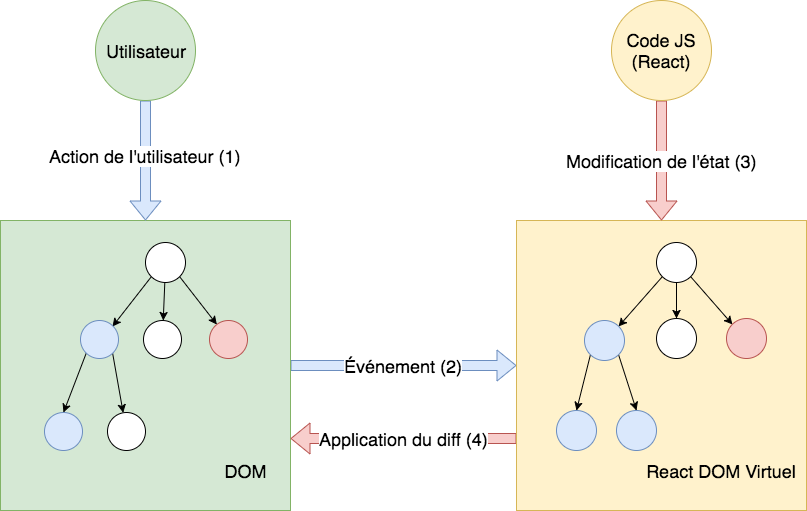
\includegraphics[scale=0.25]{images/schema-react.png}
  \caption{Schéma explicatif du principe de réconciliation de la librairie React}

\end{figure}
\end{frame}
\begin{frame}{\textit{Front-end}}{Outils d'implémentation}
  \begin{block}{JSX}
 JSX est une extension JavaScript dont l'usage est très recommandé lors du développement d'une application React.  
  \end{block}
  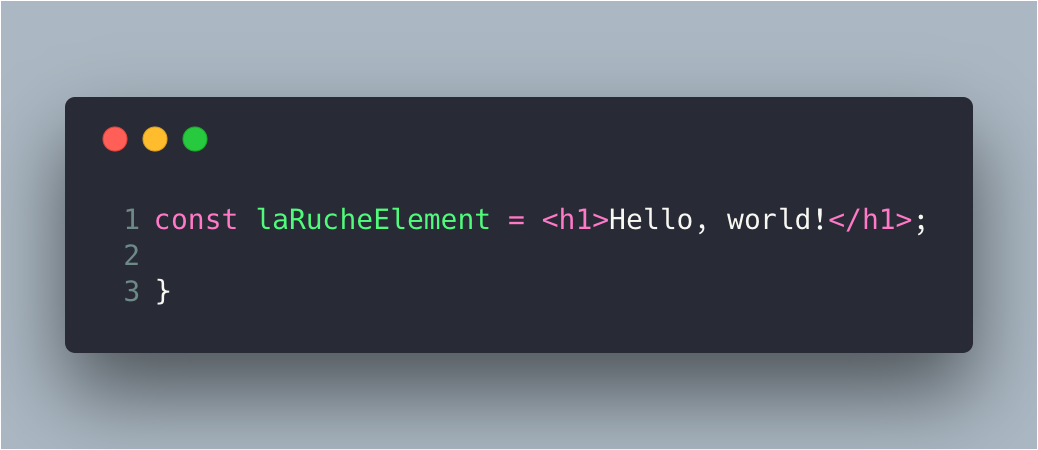
\includegraphics[scale=0.25]{images/JSX.png}

  %%Bootstrap, JS, JQuery, React
\end{frame}

\subsection{\protect\textit{Back-end}}
\begin{frame}{\textit{Back-end}}{Outils d'implémentation}
%%PHP, MySQL
  \begin{description}
    \item[Language de développement :] Serveur codé en PHP et le framework Symfony pour un système modulaire et basé sur le design pattern MVC.
    \item[Base de données :] Base de données relationnelle mise en place via MySQL, interaction avec l'ORM Doctrine.
  \end{description}
\end{frame}
%----------------------------------------------------------------------------------------
%   CONCLUSION
%----------------------------------------------------------------------------------------
\section{Conclusion}
\subsection{Écosystème décentralisé et autonome}
\begin{frame}{Écosystème décentralisé et autonome}{Conclusion}

\begin{block}{Autonomie}
Les fournisseurs sont \textbf{autonomes} : la formation des ruches et l'organisation des évènements de collecte.
\end{block}

\begin{block}{Extensibilité}
Le système est versatile et extensible : extension des ruches, augmentation de leur nombre, ajout de fonctionnalités supplémentaires, $\dots$.
\end{block}

\end{frame}

\subsection{Perspectives}
\begin{frame}{Perspectives}{Conclusion}
 \begin{itemize}
   \item Changement du nom du projet
   \item Récolte de feedback de la part d'utilisateurs potentiels
   \item Optimisation de la logistique 
   \item Implémentation de quelques fonctionnalités (inscription,paiement...)
   \item Internationalisation
 \end{itemize}
%fonctionnalités déjà discutées : paiement en ligne (CB, Paypal), politique de quasi rupture de stock et autres approches d'optimisation, etc.. (cf. section logistiques et user stories supplémentaires)
%fonctionnalités pondérées non discutées : internationalisation du site, etc...
\end{frame}
\end{document}
